\title{Exploring Graphics with WebGL}
\author{ David Moench}

\documentclass[12pt]{article}

\usepackage{amsmath}
\usepackage{graphicx}

\begin{document}
\maketitle

\begin{abstract}
These notes are intended to help me keep new material in my brain.
\end{abstract}

\newpage

\tableofcontents

\newpage

\section{3D Graphics}

\subsection{Matrices, Vectors, and Coordinates}
\paragraph{Homogeneous Vectors} 3D vectors are in the form $< x, y, z, w>$ where 
$w = 0$ means the vector is a 3D point in space, and $w = 1$ means the vector is a direction.

\paragraph{Matrices} 3D graphics deals in 4x4 matrices. There are 3 standard matrices to
understand:
\begin{description}
	\item[The Model Matrix] Move vectors from the model vector space (vectors defined
		relative to model) to the world vector space (vectors defined relative to the 
		world)
	\item[The View Matrix] Move vectors from world vector space to camera vector
		space (vectors defined relative to camera)
	\item[The Projection Matrix] Move vectors camera vector space to homogeneous
		vector space (vectors defined in a cube of what's visible). Warps the view frustum
		and all within into a cube.
\end{description}

A useful graphic: \\\\
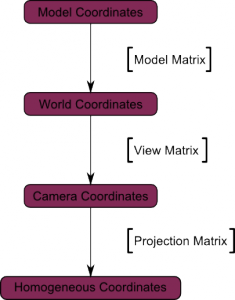
\includegraphics[width=60mm]{img/MVP_Matrices.png}
\cite{opengl}

The ModelViewProjection matrix cumulates the above 3 matrix transformations into
one.

\paragraph{Transformations} Transformations are performed by matrix multiplication.
In classic Linear Algebra form, $A\vec{x} = \vec{b}$ transfoms a vector $\vec{x}$ into 
vector $\vec{b}$. A transformation is applied to objects modeled by a collection of 
vertices by applying the transformatin to each vertex in the object.
There are 3 kinds of transformations: Translation, Rotation, and Scaling.

Translation matrices take the form: \\

$ A = \begin{bmatrix}
1 & 0 & 0 & X \\
0 & 1 & 0 & Y \\
0 & 0 & 1 & Z \\
0 & 0 & 0 & 1
\end{bmatrix}$ \\

Where X, Y, and Z are the amount by which the vector operand's x, y, and z 
components are translated. For example, translate a vector position at
$<0,0,0>$ 2 units in the x and y directions: \\

$
\begin{bmatrix} 1 & 0 & 0 & 2 \\ 0 & 1 & 0 & 2 \\ 0 & 0 & 1 & 0 \\ 0 & 0 & 0 & 1
\end{bmatrix}\begin{bmatrix} 0 \\ 0 \\ 0 \\ 1 \end{bmatrix} = 
\begin{bmatrix} 2 \\ 2 \\ 0 \\ 1 \end{bmatrix}
$ \\

Notice that the resulting vector is also a position vector (4th element is 1).
Applying a translation to a direction vector $<x,y,z,0>$ does not
affect it. 

Scaling matrices take the form: \\

$ A = \begin{bmatrix}
X & 0 & 0 & 0 \\
0 & Y & 0 & 0 \\
0 & 0 & Z & 0 \\
0 & 0 & 0 & 1
\end{bmatrix}$ \\

Where X, Y, and Z represent the scaling factor applied to the operand vector's
x, y, and z components. Notice the components can be scaled independently
in one scaling transformation. Also the operand vector's $w$ status is
unaffected.

% TODO - Rotation Matrices

Multiple transformations can be cumulated into a single matrix via multiplication.
For example: 

$TransformationMatrix = ScaleMatrix * RotateMatrix * TranslateMatrix$

Notice the 3 transformations will be performed in order from left to right.

\section{WebGL}

\paragraph{Overview} WebGL is a javascript API for rendering 3D content on an
HTML5 canvas element. Allows faster rendering by using a computer's GPU.

\subsection{Components of a WebGL Application}
\begin{enumerate}
	\item Create canvas element
	\item Initialize a WebGL javascript context for it.
	\item Create buffers of vertices to be rendered
	\item Create matrices for transformations
	\item Create shaders
	\item Initialize shaders with params
	\item Draw 
\end{enumerate}
\cite{upandrunning}

\subsection{Buffers}
Buffers are data structures that hold collections of vertices. They are loaded
onto the GPU so future drawing operations on those vertices can be done fast.
Some types: \verb|ARRAY_BUFFER|,  \verb|ELEMENT_ARRAY_BUFFER|.

Buffers must be bound to the WebGL context's  \verb|ARRAY_BUFFER| member (The "current
buffer"), and only one buffer may be bound and operated upon at any time.
Binding loads them onto the GPU. 

To load vertex data into a buffer: Create an array, convert to a Float32Array
object, and load into the current  \verb|ARRAY_BUFFER| via .bufferData(). Also 
need to specify the item size (number of array fields per vertex: 3) and
number of items (number of distint vertex positions). There is a seperate
current  \verb|ELEMENT_ARRAY_BUFFER|.

An \emph{element array buffer} specifies vertices in an array buffer that will
be used to draw shapes. For example, you want to draw a square composed of 2
triangles but don't want to use triangle strips. Create an array buffer $A$ of 4 
vertices, then an array element buffer of 6 indicies (0,1,3, 0,2,3) in $A$ to 
create the 2 triangles that make the square. 

\subsection{Shaders}
Shader programs are a mechanism for representing your models in a way the GPU can
understand. Shader source code is written in GLSL not javascript.

\begin{description}	
	\item[Vertex Shader] Handles conversion of 3D vertex coordinates to 2D clipspace
		coordinates. Called for every verted - can apply model-view and projection 
		matrices to collections of vertices much faster on the GPU than through a javascript loop.
		Outputs \emph{varying} variables (eg:  \verb|gl_Position| - a vertex's final coords).
	\item[Fragment Shader] Handles coloring of fragments (triangle planes formed by
		3 vertices). Called once for each pixel of the image. Performs linear interpolation
		between verteces => fills in spaces and creates color gradients.
\end{description}

There are 3 qualifiers for shader variables: \emph{Uniforms}, \emph{Attributes}, and \emph{Varyings}. 
Uniforms are the same across the entire frame being rendered (eg: projection and model-view matrices). 
Attributes are input values that vary from vertex to vertex, and are only accessible by 
vertex shader. Varyings are declared in vertex shader to be shared with fragment shader.

Here's a useful diagram of the rendering pipeline \cite{learnwebgl}: \\
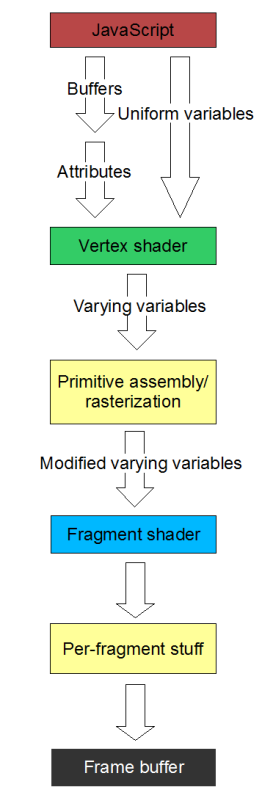
\includegraphics[width=60mm]{img/simple-rendering-pipeline.png}

\paragraph{How to get color to the fragment shader?} You can't pass data to frag shader 
directly. Define a \emph{varying} variable in the vector shader that will be passed
along to the fragment shader for interpolation. 

\section{Useful Libraries}
\paragraph{Three.js} %TODO
\paragraph{glMatrix} For optimized matrix and vector math.

\begin{thebibliography}{9}
	\bibitem{opengl} http://www.opengl-tutorial.org
	\bibitem{learnwebgl} http://learningwebgl.com
	\bibitem{upandrunning} WebGL: Up And Running
	\bibitem{quickref} \verb|http://www.khronos.org/files/webgl/webgl-reference-card-1_0.pdf|
\end{thebibliography}

\end{document}
